% A listing of the contents of each file supplied as Supporting Information
% should be included. For instructions on what should be included in the
% Supporting Information as well as how to prepare this material for
% publications, refer to the journal's Instructions for Authors.

% The following files are available free of charge.
% \begin{itemize}
% \item Filename: brief description
% \item Filename: brief description
% \end{itemize}

Supplementary figures:
\begin{itemize}
\item \cref{tab:table-mult}
\item \cref{fig:steps-v-corr}
\item \cref{tab:table-versions}
\item \cref{fig:structs-v-corr-id-zemu-12-60000-rscript-validated-t14}
\item \cref{fig:structs-v-corr-WildTypeComplex-ddg-monomer-16-003-zemu-2}
\item \cref{fig:wildtypecomplex-scores-complete}
\item \cref{fig:spear-corr-rmsd-error}
\item \cref{fig:t14-mean-ensemble}
\item \cref{tab:table-ref}
\item \cref{tab:table-antibodies}
\item \cref{fig:t14-fits-feats}
\end{itemize}

\subimport*{figs-and-tables/}{table-mult}
\subimport*{figs-and-tables/}{steps-v-corr}
\subimport*{figs-and-tables/}{table-versions}
\subimport*{figs-and-tables/}{table-antibodies}
\subimport*{figs-and-tables/}{structs-v-corr-id-zemu-12-60000-rscript-validated-t14}
\subimport*{figs-and-tables/}{structs-v-corr-WildTypeComplex-ddg-monomer-16-003-zemu-2}

\begin{figure}
  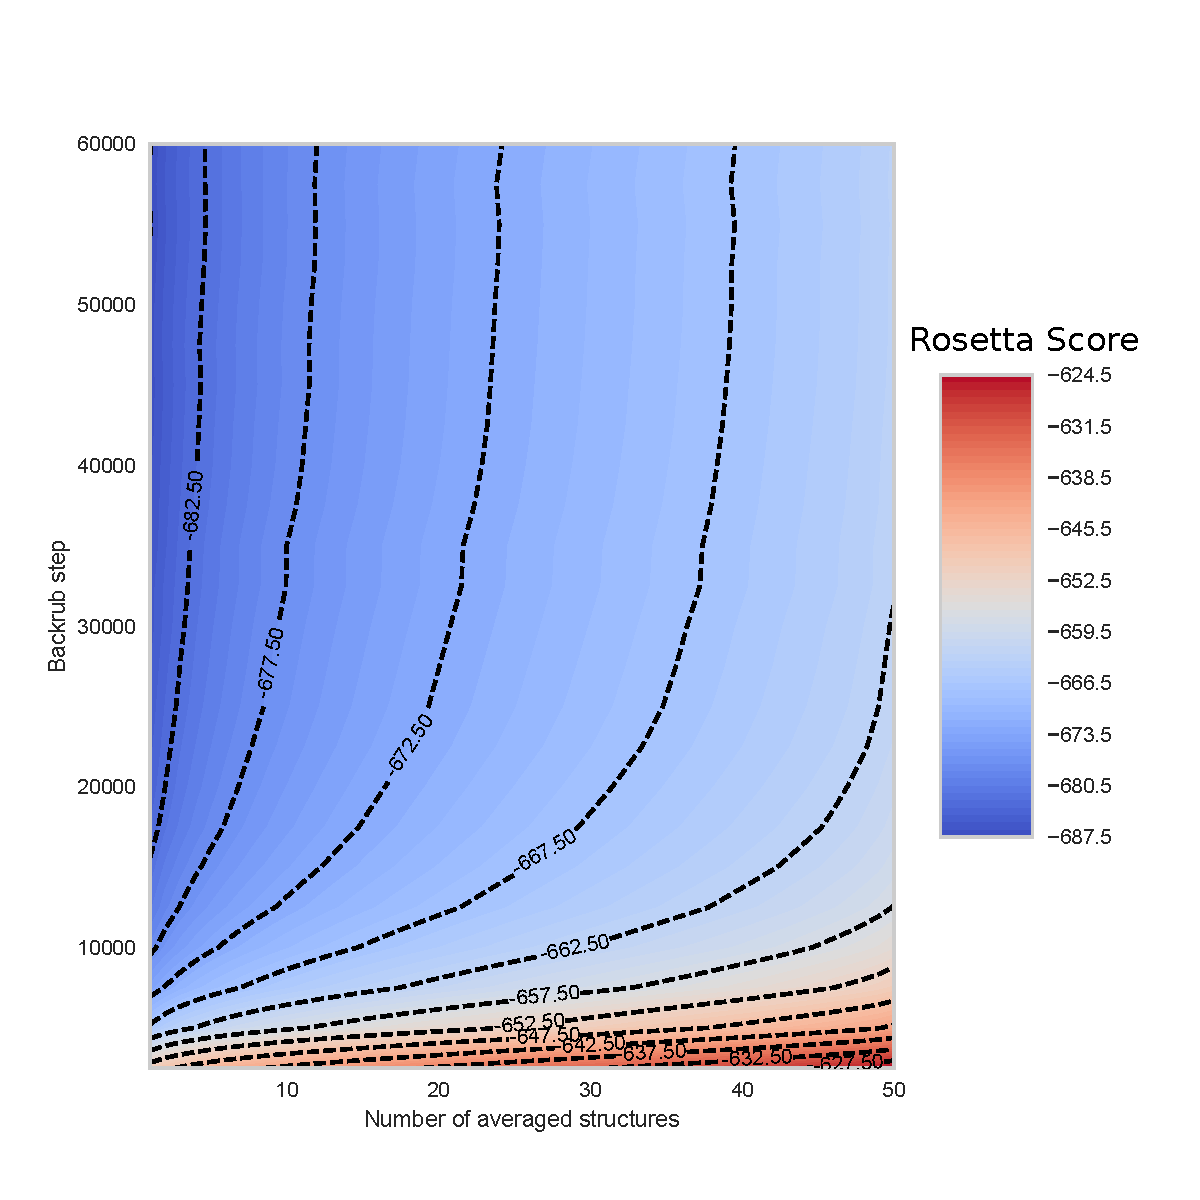
\includegraphics[width=\textwidth,keepaspectratio]{figures/wildtypecomplex-scores-complete.pdf}
  \caption{
    Contour plot showing the effect of backrub sampling on the average wild-type complex score, for varying numbers of averaged models.
  } \label{fig:wildtypecomplex-scores-complete}
\end{figure}

\begin{figure}
  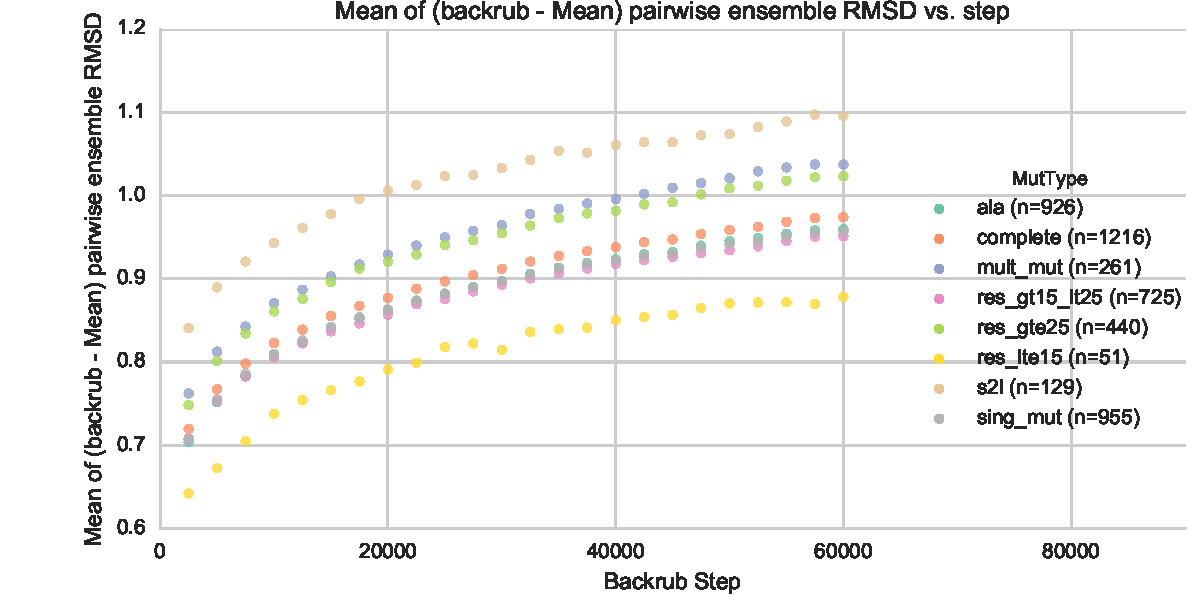
\includegraphics[width=\textwidth,keepaspectratio]{figures/t14-mean-ensemble-error.pdf}
  \caption{
    Mean backrub ensemble RMSD vs. backrub steps.
  } \label{fig:t14-mean-ensemble}
\end{figure}

\begin{figure}
  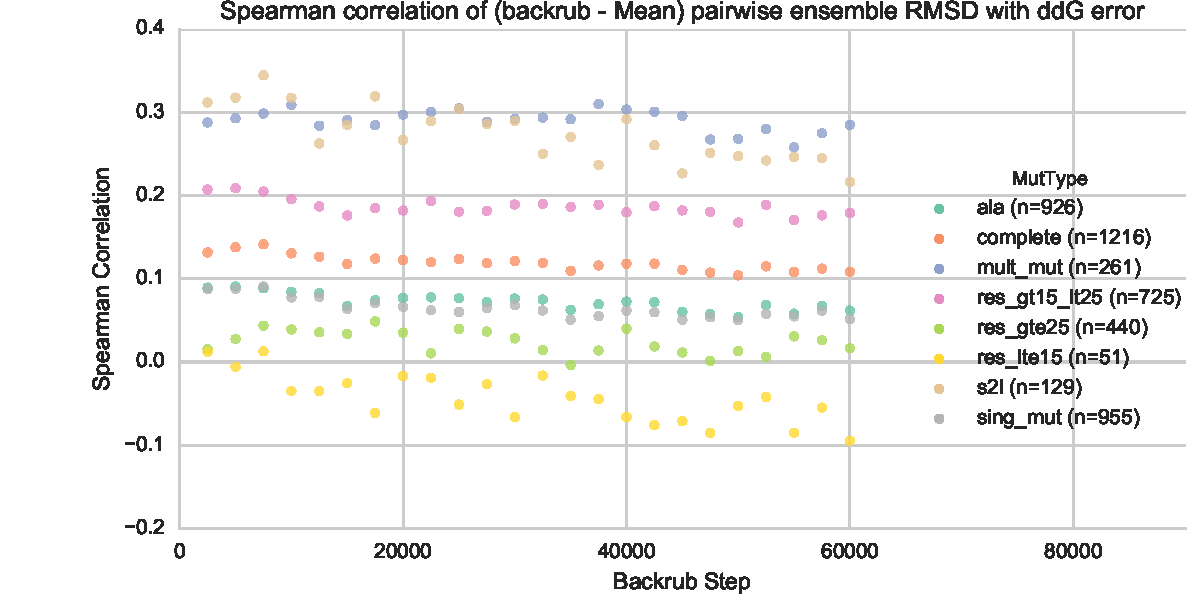
\includegraphics[width=\textwidth,keepaspectratio]{figures/t14-spear-corr.pdf}
  \caption{
    Scatter plot showing the average Spearman correlation of ddG prediction error v. mean backrub ensemble RMSD, v. backrub steps.
    As mean backrub ensemble RMSD increases (\cref{fig:t14-mean-ensemble}), we don't see any significant change in correlation between mean ensemble RMSD and ddG error.
    This demonstrates that mean pairwise backrub ensemble RMSD is not an effective metric to measure the degree to which we have sampled ``enough''.
  } \label{fig:spear-corr-rmsd-error}
\end{figure}

\begin{figure}
  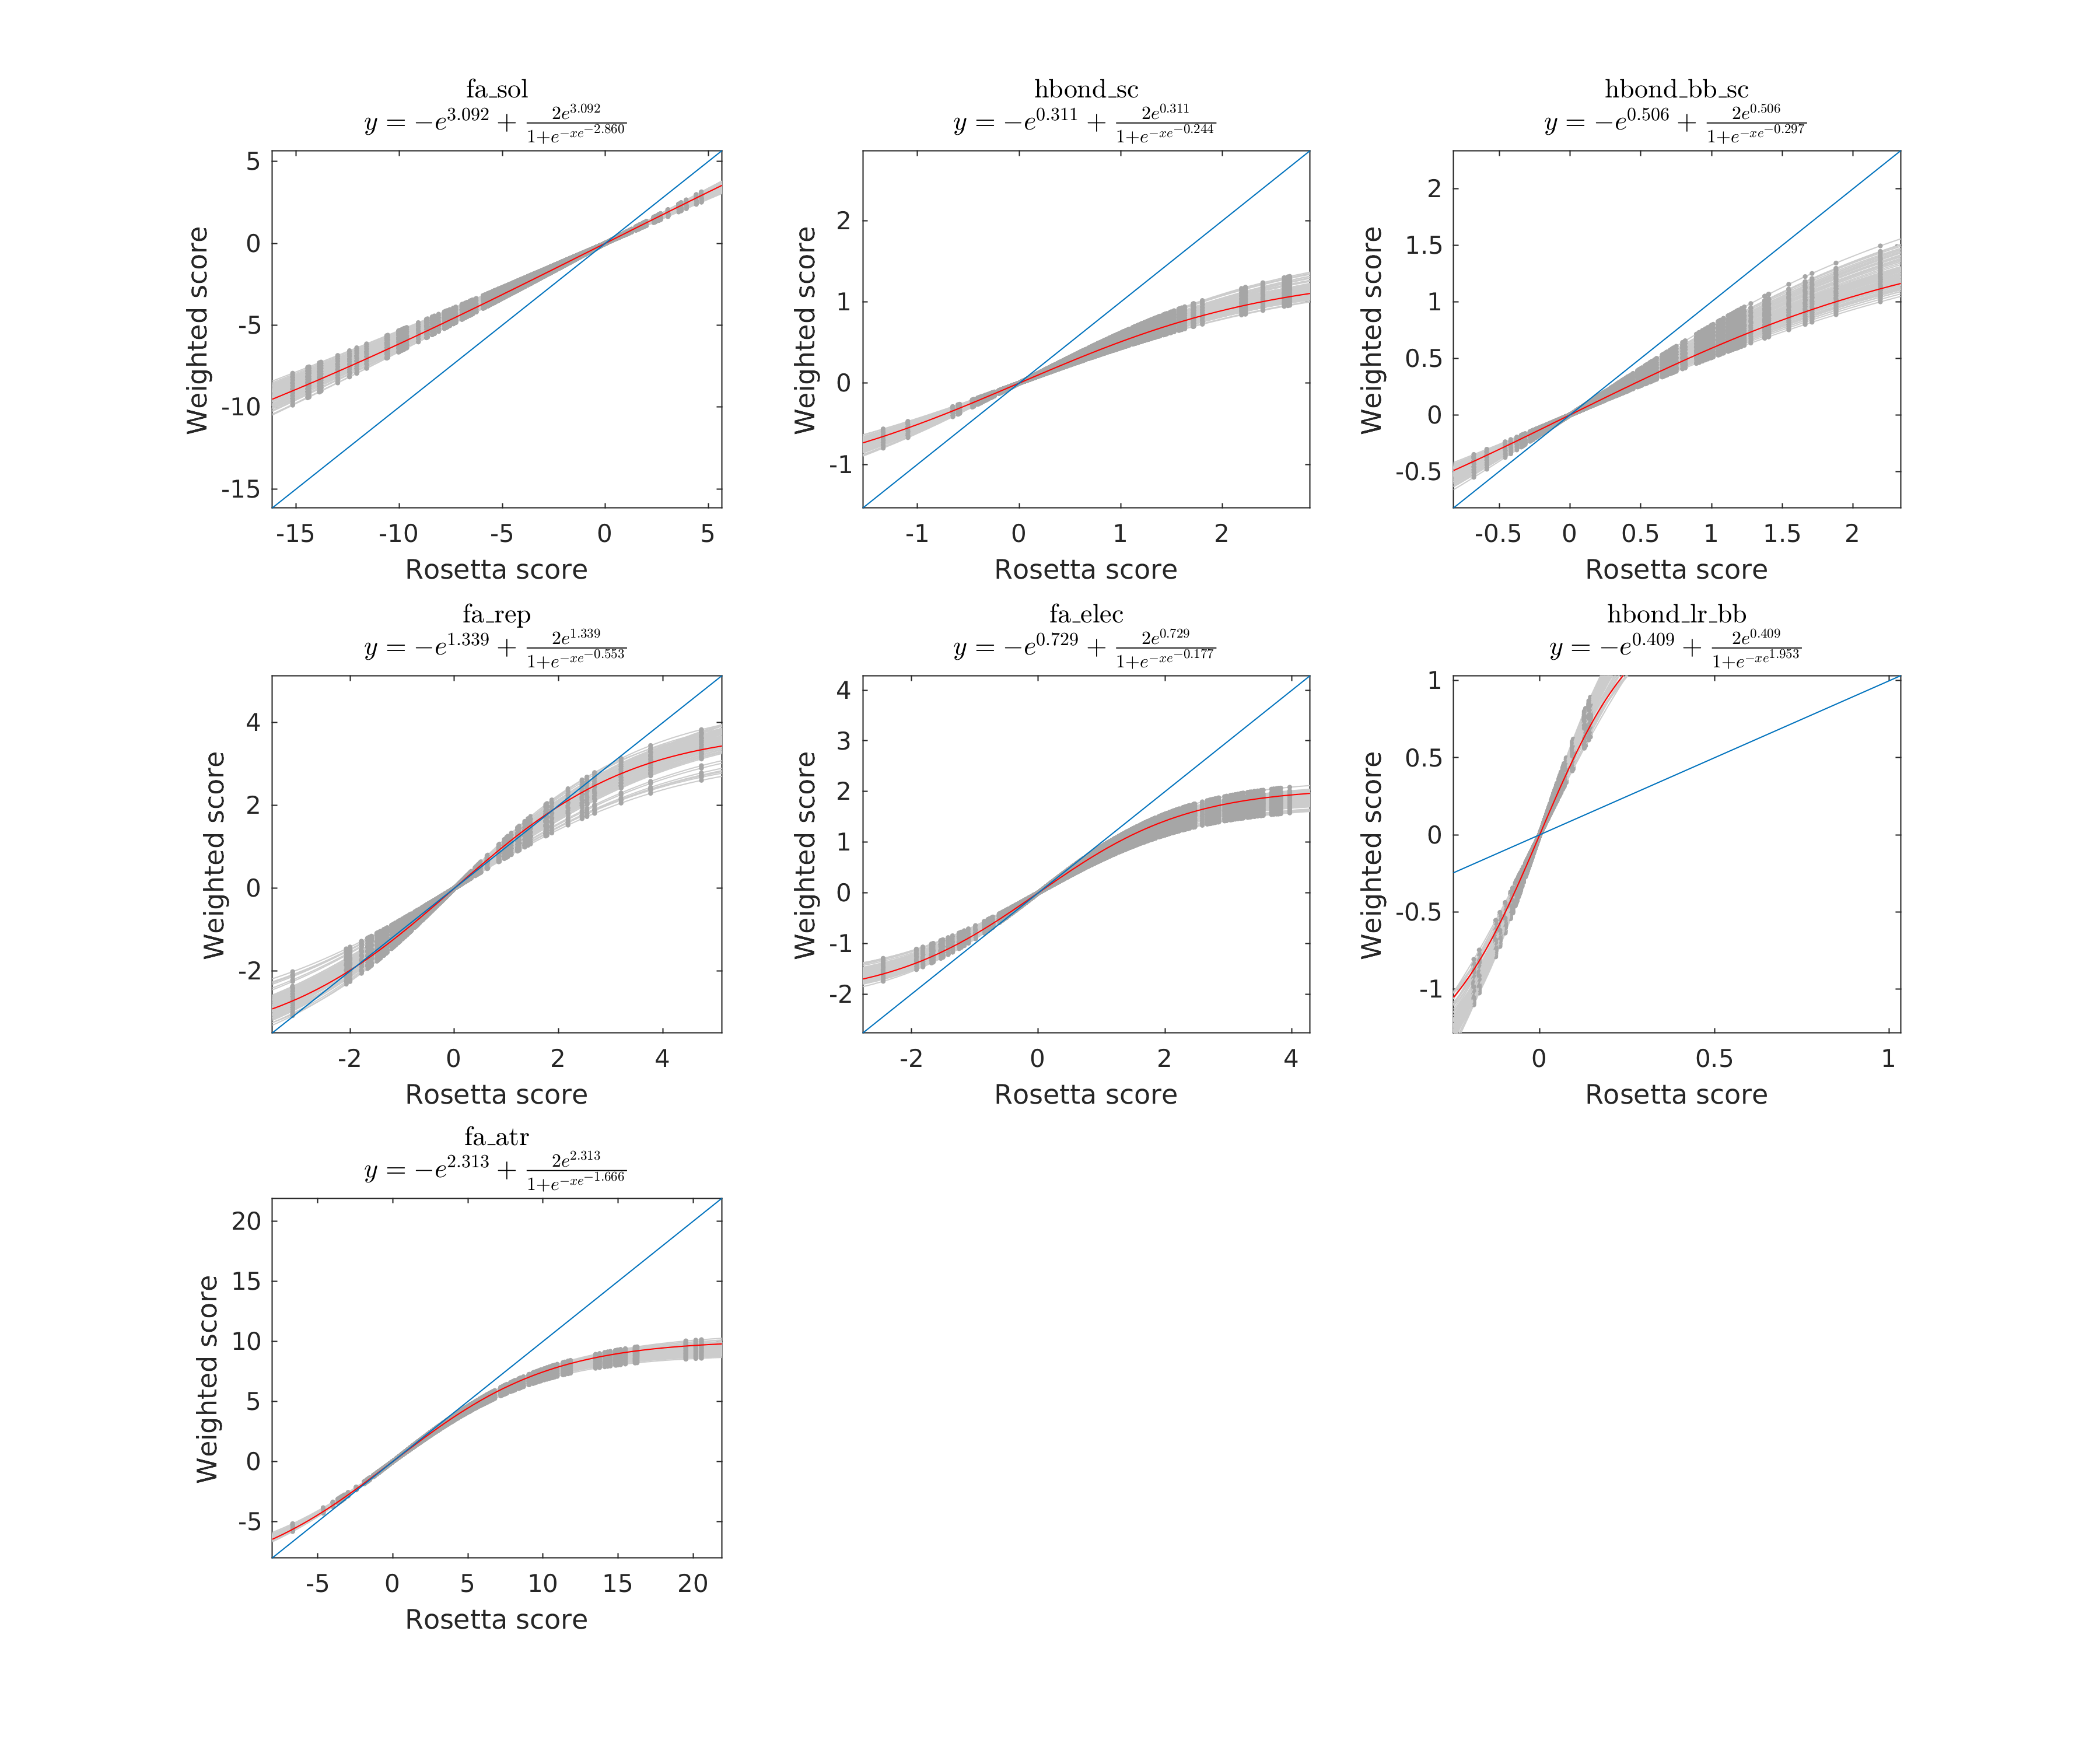
\includegraphics[width=\textwidth,keepaspectratio]{figures/zemu-sigmoid2-tal-feats.png}
  \caption{
    Markus' most recent fit score function functions
  } \label{fig:t14-fits-feats}
\end{figure}

\begin{figure}
  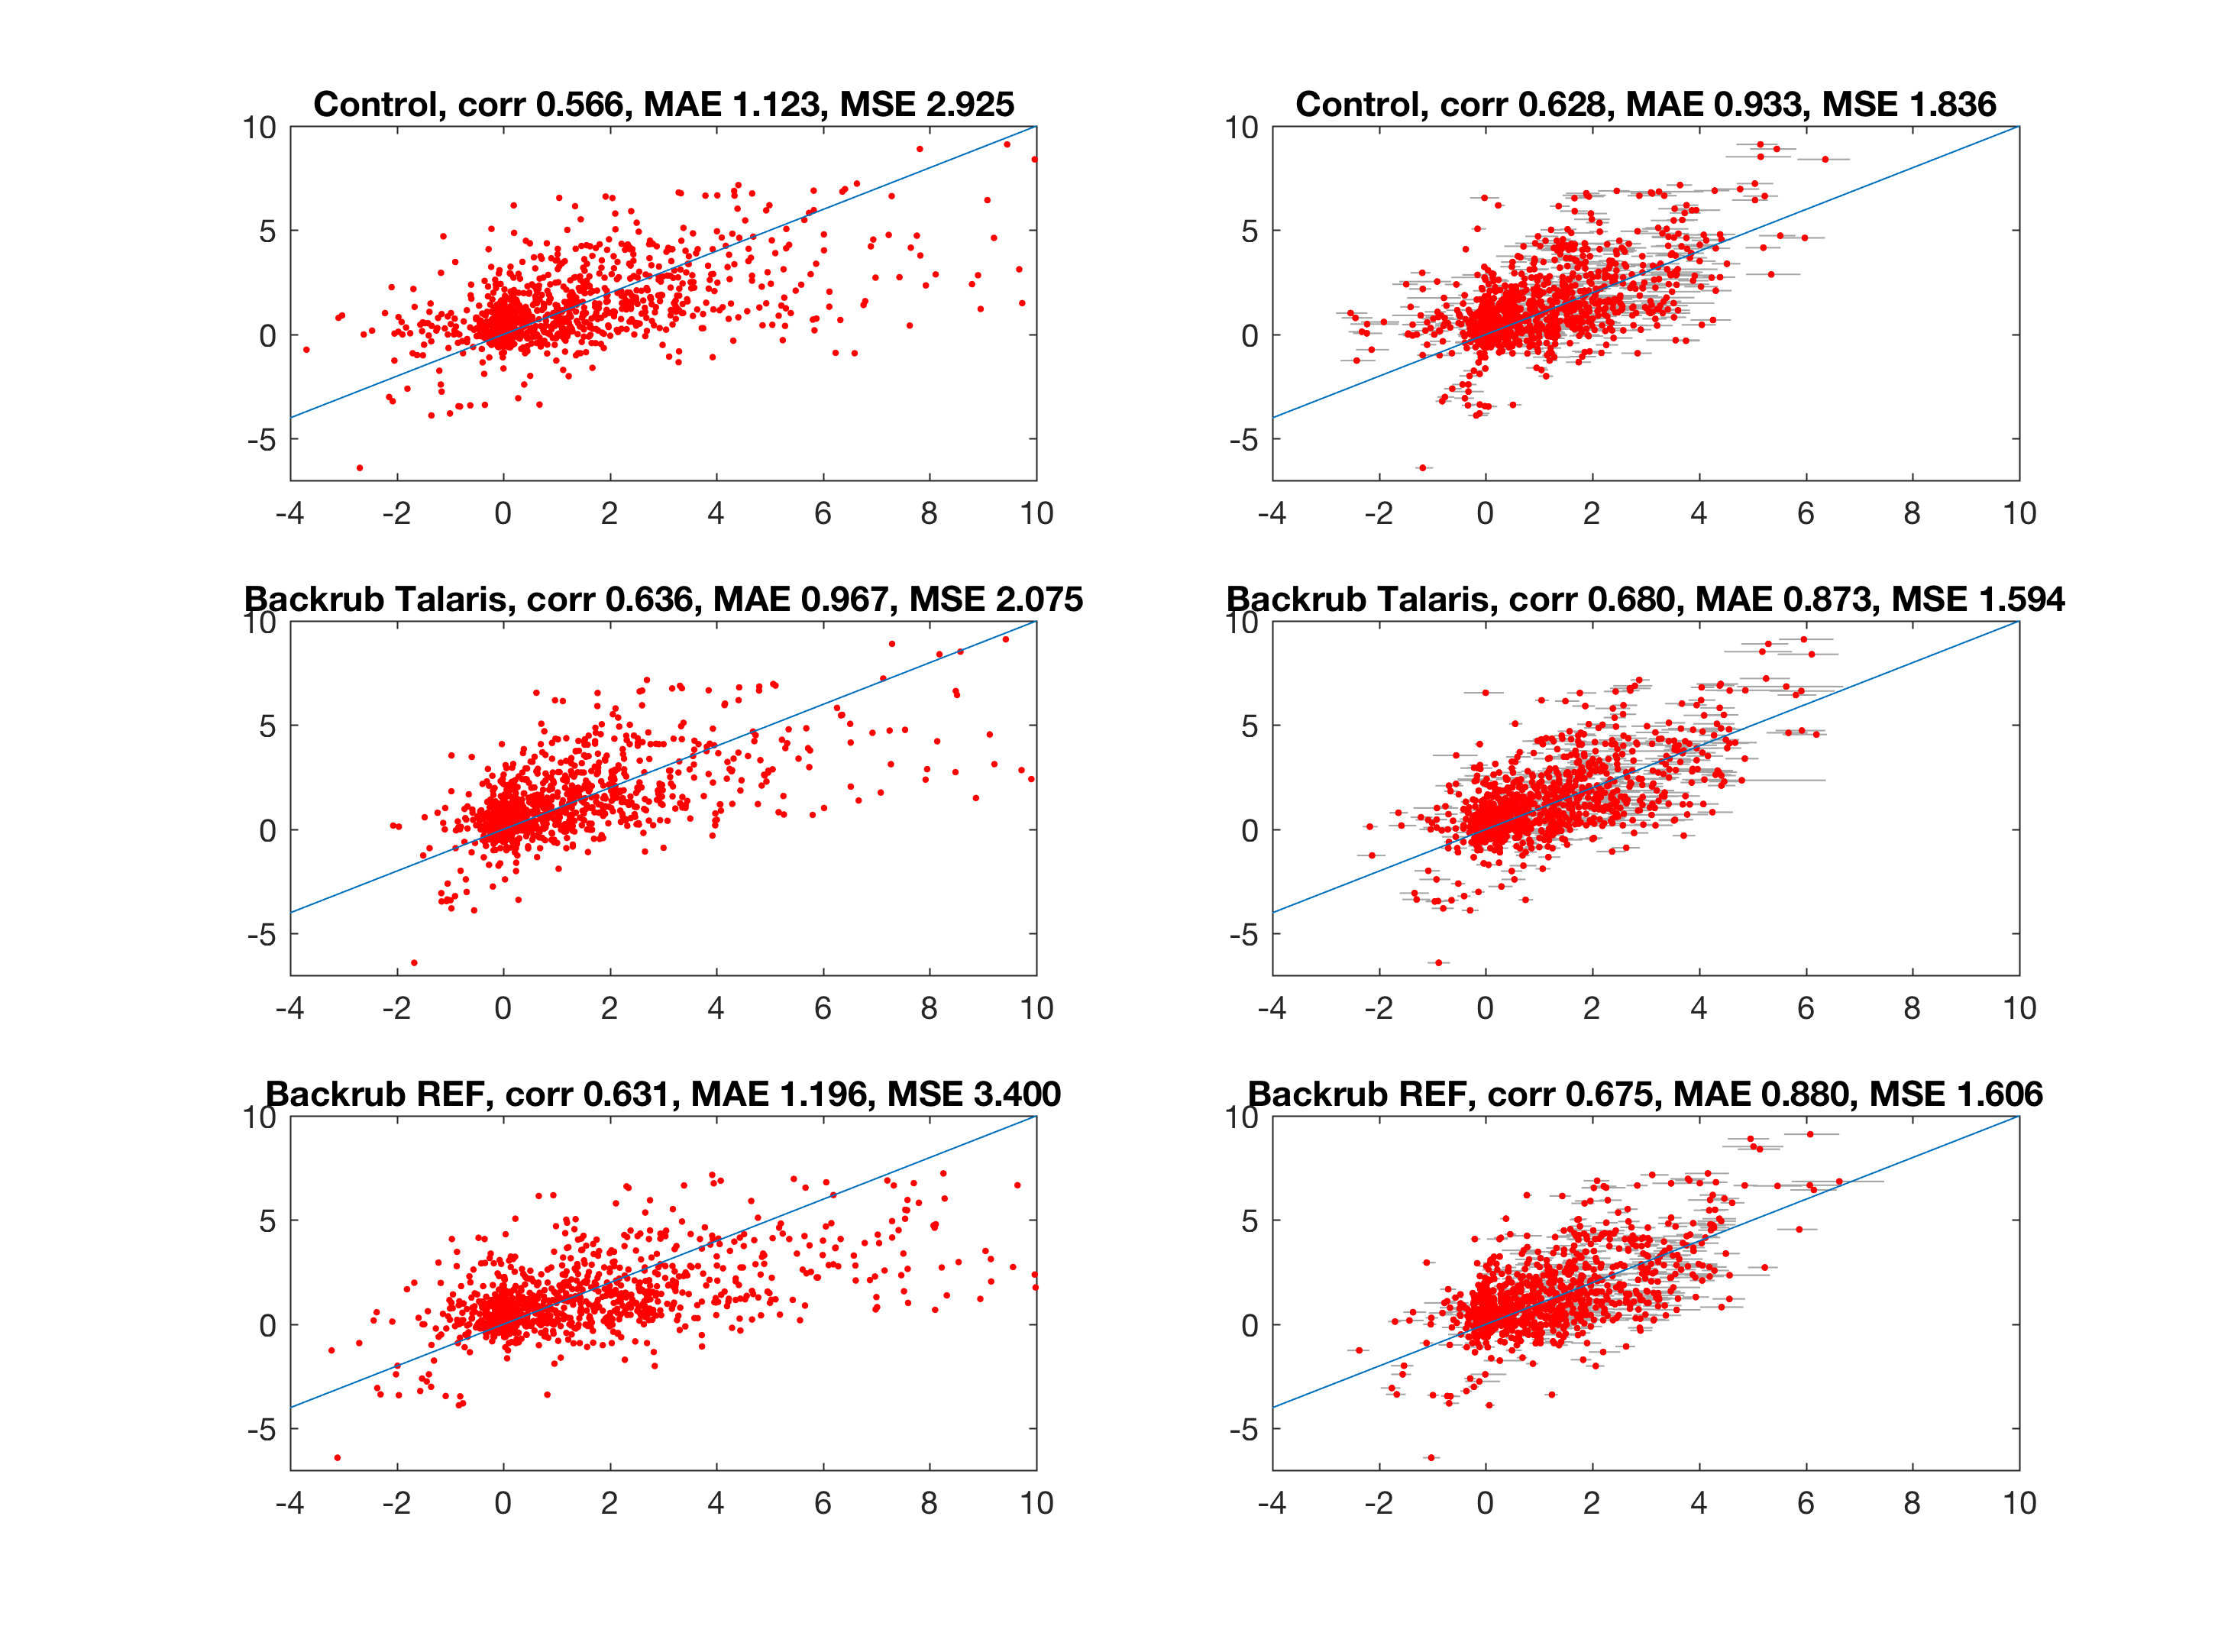
\includegraphics[width=\textwidth,keepaspectratio]{figures/zemu-sigmoid2-corrs.png}
  \caption{
    Left: standard, non-fitted predictions vs. experimental \ddg\ values. Right: Fit predictions vs. experimental data. Top: Control (no backrub) predictions. Middle: Backrub/talaris. Bottom: Backrub/REF.
  } \label{fig:t14-fit-scatter}
\end{figure}

\subimport*{figs-and-tables/}{table-ref}